% !TeX root = ../main.tex
% !TEX root = ../main.tex
% -*- root: ../main.tex -*-
% -*- program: pdflatex -*-
\chapter{利用样条插值方法对~MRPC~进行刻度}

~MRPC-TOF~直接测量的信息包括原始的飞行时间和过阈时间(~time-over-threshold~,简称~TOT~)。为了得到精确的飞行时间信息,还需要对时幅游走、过大信号、粒子在对数条上的传播时间,以及在电子学电缆等的时间延迟等因素进行刻度和修正,还要进行离线分析。为了得到良好的时间分辨,必须对不同粒子的样本进行离线的刻度和修正,得到相应的刻度常数,再对原始数据进行重建从而得到飞行时间探测器的性能。
%\begin{comment}
~MRPC-TOF~的离线刻度是通过比较测量时间~$t_{mea}=t_{raw}-t_{0}-t_{cor}$~与带电粒子从对撞顶点到击中~MRPC-TOF~的预期飞行时间~$t_{exp}=L/\beta c$~来比较,其中~$t_{0}$~是事例的起始时间,~$t_{cor}$~是时间的修正项;~c~是真空中的光
速,$\beta=p/\sqrt{p^2+m^2}$是带电粒子的飞行时间,~m~是粒子的质量,飞行长度~L~和动量~P~是通过主漂移室(~MDC~)测量得到的。飞行时间修正项~$t_{cor}$~是过阈时间~TOT~和~Z~向击中位置的函数。
%\end{comment}
对于每一个读数条,每个读出单元定义:
%\begin{equation}
\begin{displaymath}
\chi^2(counter,readout)=\sum\limits_{event}(t_{mea}-t_{exp})^2
\end{displaymath}
%\end{equation}
通过分析大量的事例样本,进行反复迭代,利用最小~$\chi^2$~方法,刻度常数项可以通过~$\partial\chi^2/\partial P_{i}=0$~得到。在重建中,利用刻度得到的刻度常数对原始的飞行时间信息进行重建,就可以得到经过刻度修正得到的飞行时间信息。

STAR~实验MRPC采用的是样条插值(~spline Fit~)刻度的方法。因此本文也对~BESIII~的~MRPC~进行了样条插值方法的研究。
本章主要介绍样条插值方法。分两部分介绍:先对过阈时间进行插值,之后对击中位置修正;先对击中位置进行修正,之后对过阈时间进行插值。并进行了一定的结果比较,发现先修正击中位置,然后对过阈时间进行插值的结果比另一种方法好。

样条插值方法优点:光滑性好,且低阶就能拟合的很好。高能所集群下的~root~中有关于~TSpline~的类包,可以利用它完成样条插值的拟合。

本章数据选用的是~2016~年5月24日到5月30日这期间~BESIII~对撞数据中的~Bhabha~事例。选用~Bhabha~事例是因为它事例量大,易于挑选,纯度高,适合做刻度样本。

%%%%%%%%%%%%%%%%%%%%%%%%%%%%%%%%%%%%%%%%%%%%%%%%%%%%%%%%%%%%%%%%%%%%%%%%%%%%%%
\section{修正击中位置前进行插值}
%%%%%%%%%%%%%%%%%%%%%%%%%%%%%%%%%%%%%%%%%%%%%%%%%%%%%%%%%%%%%%%%%%%%%%%%%%%%%%

本节以挑选的~Bhabha~事例中击中MRPC-TOF读数条位置在~MRPC~中模块编号为~55~,对数条编号为~7~这一个读数条为例。具体做法,就是先对过阈时间进行插值修正,之后对得到的结果再次对击中位置进行修正得到最终的时间分辨等刻度信息。
\subsection{等事例数分~bin~拟合}
\begin{itemize}
    \item 以过阈时间的大小为量对所选的事例数进行等事例数分~bin~
    \item 对于每个~bin~区间,进行拟合
    \item 对于上一步得到的中心值进行插值,得到插值的刻度常数
    \item 利用上一步得到的刻度常数,对时间信息进行修正 
\end{itemize}
等事例数分~bin~的原因是时间随过阈时间的分布是不均匀的。在过阈时间很小或者很大的时候事例数很少,如果采用等区间分~bin~的话,会出现比较大的误差棒。分~bin~完成后,发现一个~bin~内时间有两个峰值。图~\ref{fig:ScatterDiagram}~是时间对~TOT~的分布,图~\ref{fig:cutScatterDiagram}~是图~\ref{fig:ScatterDiagram}~截取的一部分。

\begin{figure}[htbp]
\begin{minipage}[t]{0.5\linewidth}
%\centering
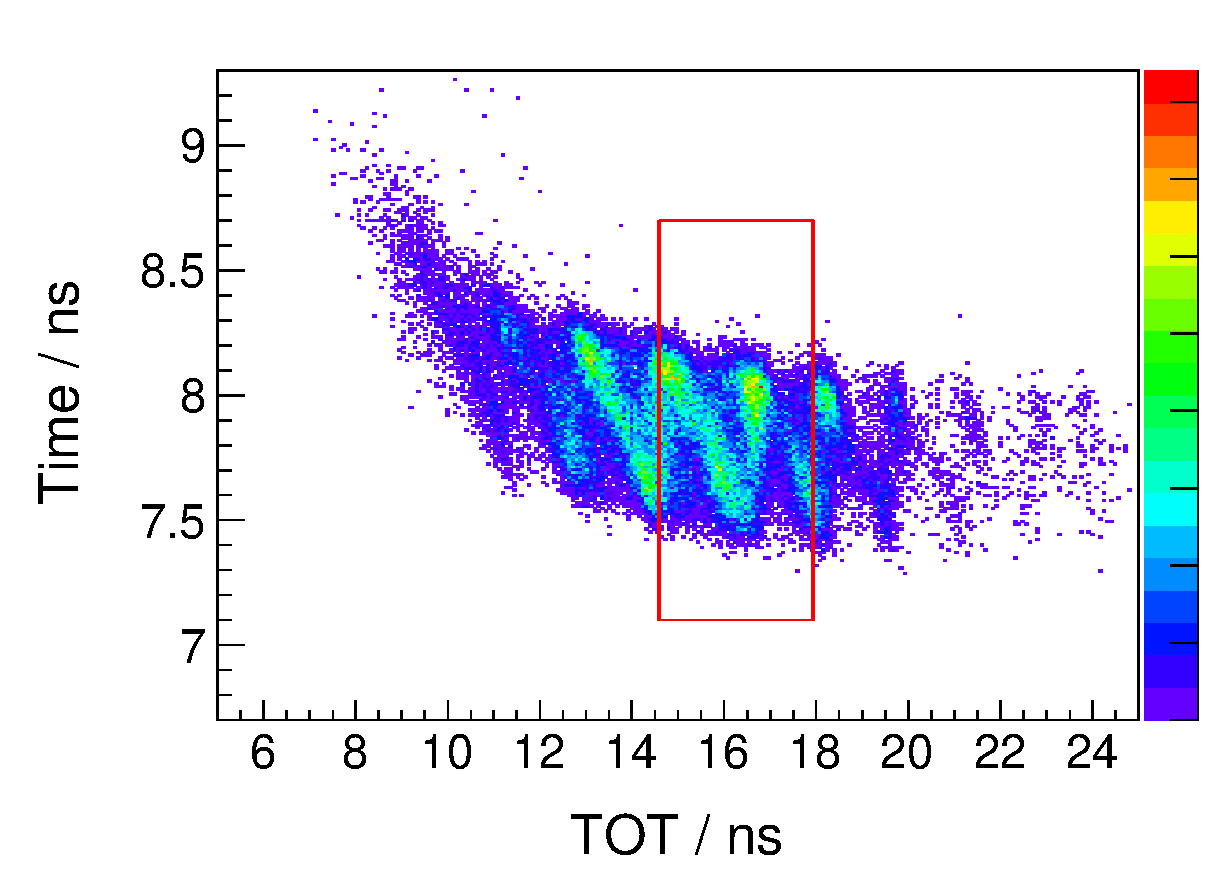
\includegraphics[width=0.9\textwidth]{chap2/ScatterDiagram.eps}
\subcaption{时间对TOT的分布}
\label{fig:ScatterDiagram}
\end{minipage}%
\hfill
\begin{minipage}[t]{0.5\linewidth}
%\centering
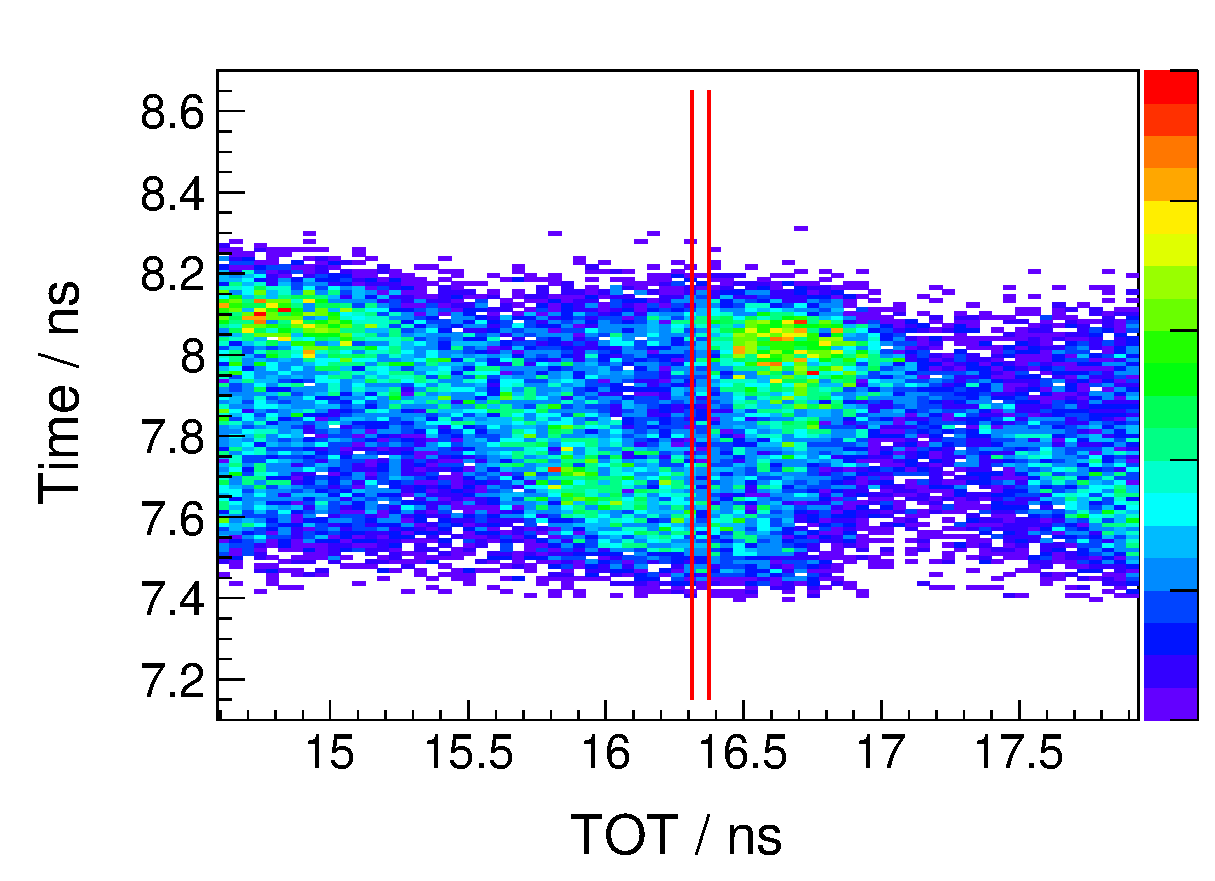
\includegraphics[width=0.9\textwidth]{chap2/cutScatterDiagram.eps}
\subcaption{截取时间对TOT的分布}
\label{fig:cutScatterDiagram}
\end{minipage}
\caption{时间对TOT的分布}
%\label{fig:Diagram}
\end{figure}

\begin{figure}[htbp]
\centering
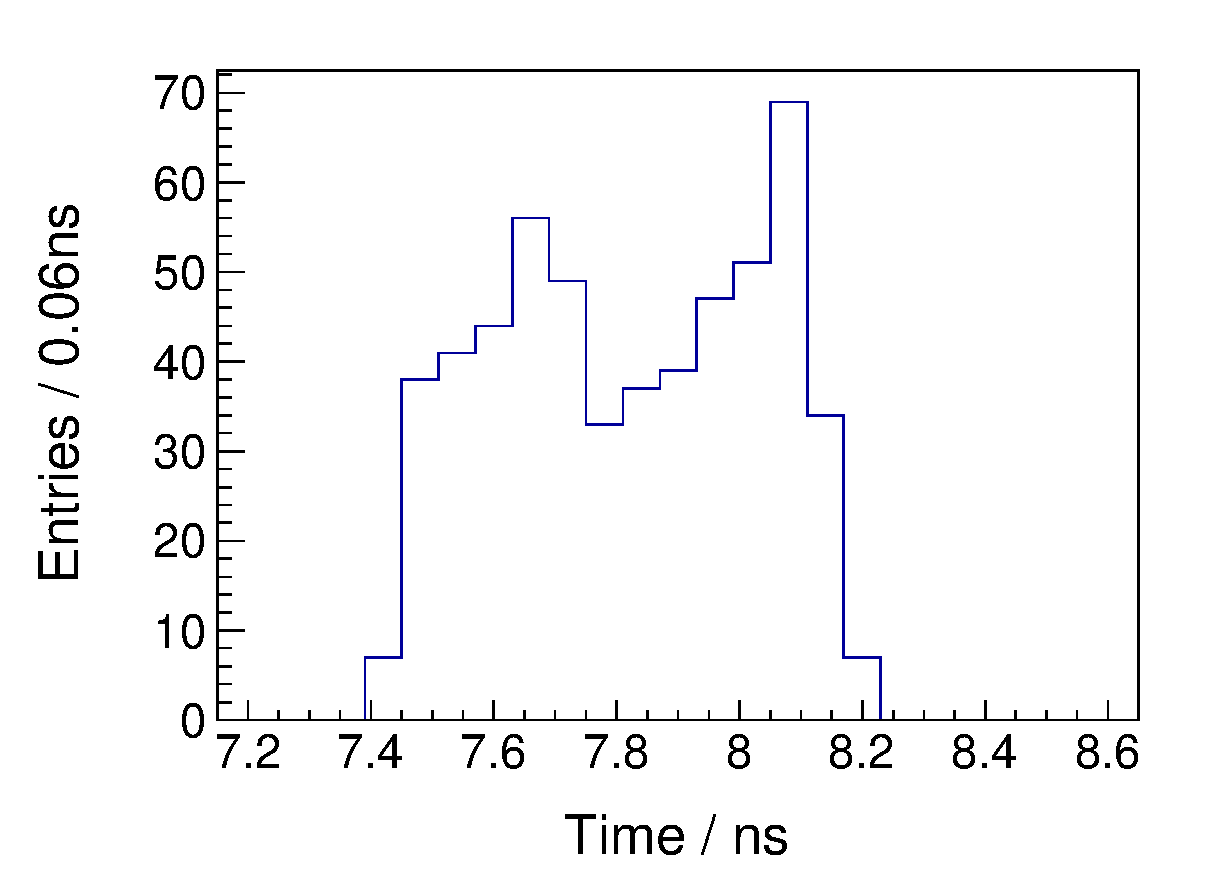
\includegraphics[width=0.5\textwidth]{chap2/onebinTime.eps}
\caption{截取一个bin的时间分布(对应两个峰值)}
\label{fig:onebinTime}
\end{figure}

图~\ref{fig:onebinTime}~是一个bin内的时间分布,可以明显看出具有双峰。对此,找不到合适的函数可以在一个区间内得到一个合适的中心值。

\subsection{两个高斯拟合和单个高斯拟合}

图~\ref{fig:double-ScatterDiagram}~,~\ref{fig:single-ScatterDiagram}~分布是对每个~bin~用两个高斯和一个高斯函数拟合后得到的中心值的分布

\begin{figure}[!h]
\begin{minipage}[!h]{0.5\linewidth}
%\centering
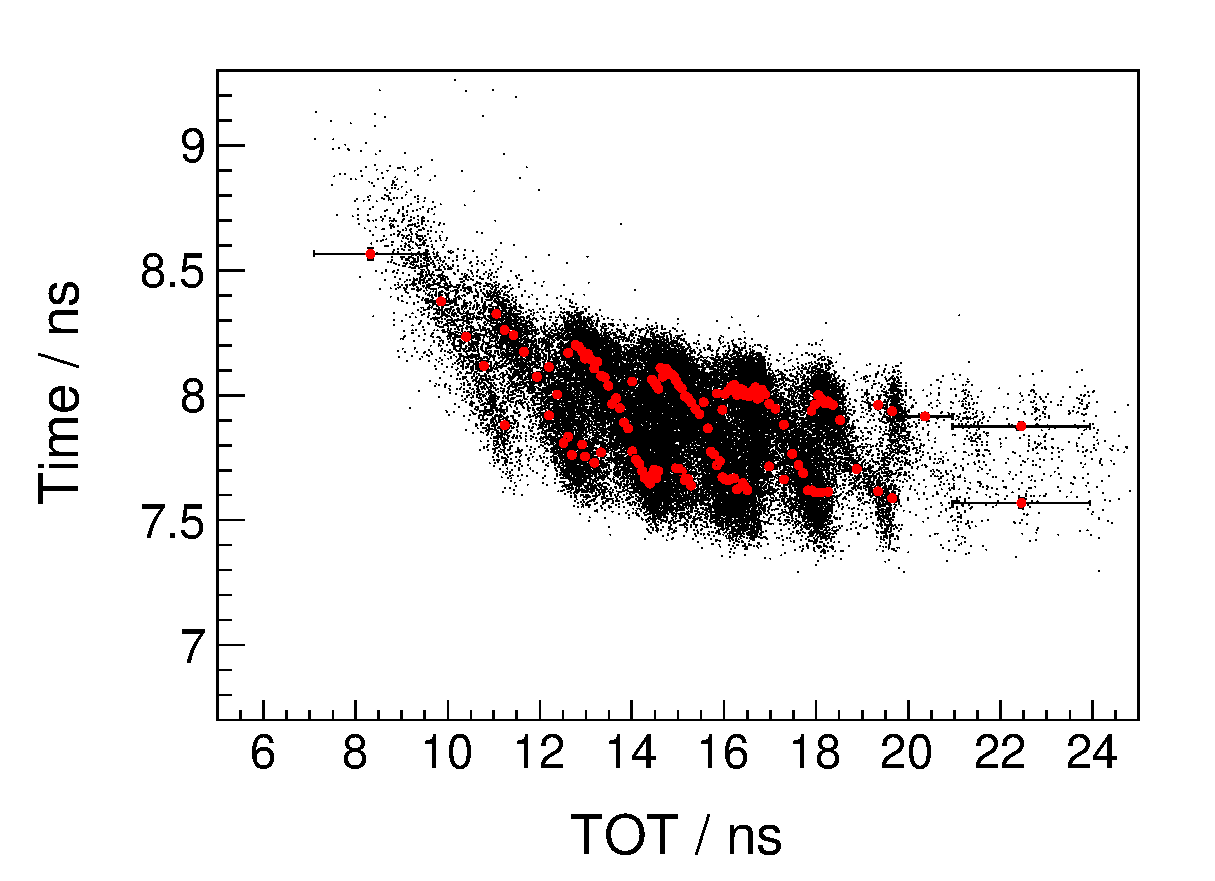
\includegraphics[width=0.95\textwidth]{chap2/double-ScatterDiagram.eps}
\subcaption{两个高斯拟合后的graph图}
\label{fig:double-ScatterDiagram}
\end{minipage}%
\hfill
\begin{minipage}[!h]{0.5\linewidth}
%\centering
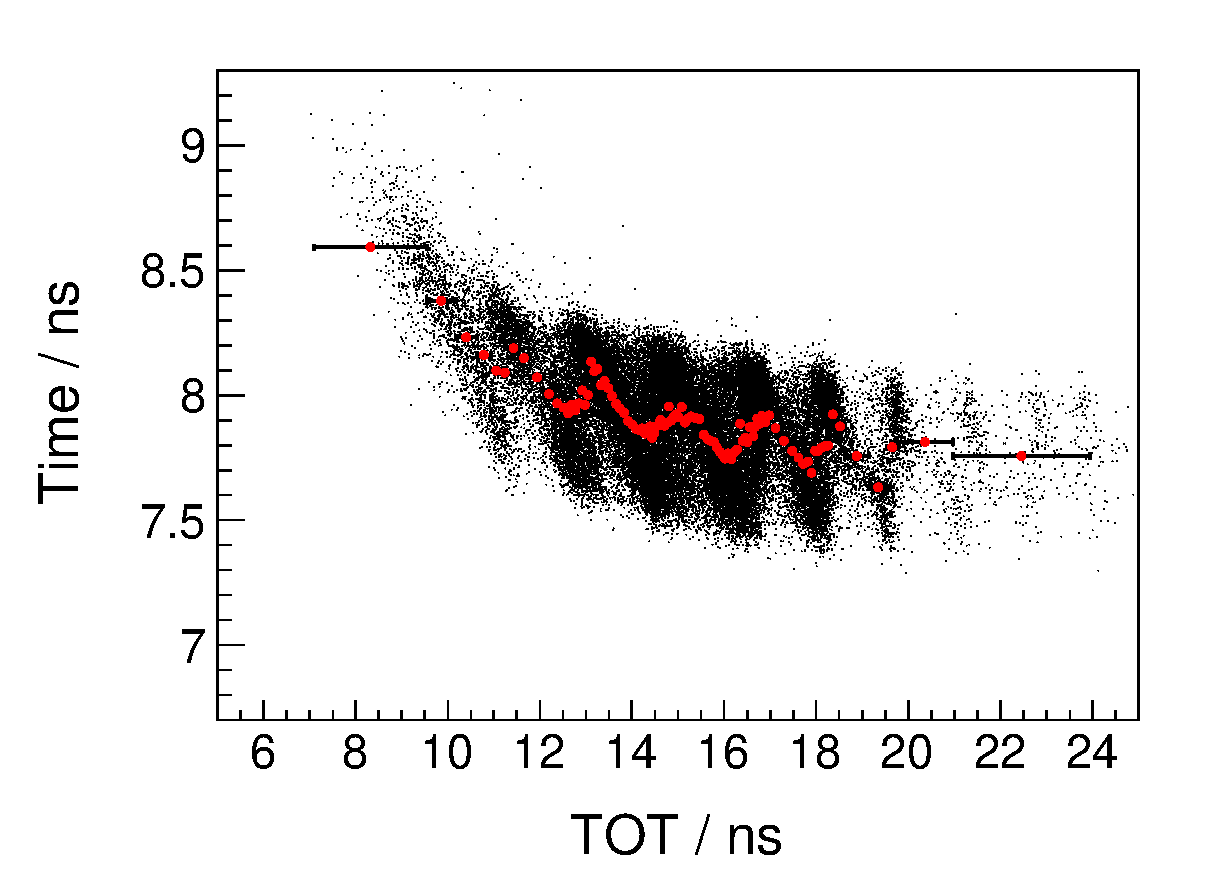
\includegraphics[width=0.95\textwidth]{chap2/single-ScatterDiagram.eps}
\subcaption{一个高斯拟合后的graph图}
\label{fig:single-ScatterDiagram}
\end{minipage}
\caption{高斯拟合后的graph}
\end{figure}

图~\ref{fig:double-leftspline}~第一种做法的样条插值曲线,对于每个~bin~的时间的中心值取相对比例高的。图~\ref{fig:single-leftspline}~第二种做法的样条插值曲线。对比看出,右图的拟合更符合原来散点的分布情况。

\begin{figure}[!h]
\begin{minipage}[!h]{0.5\linewidth}
%\centering
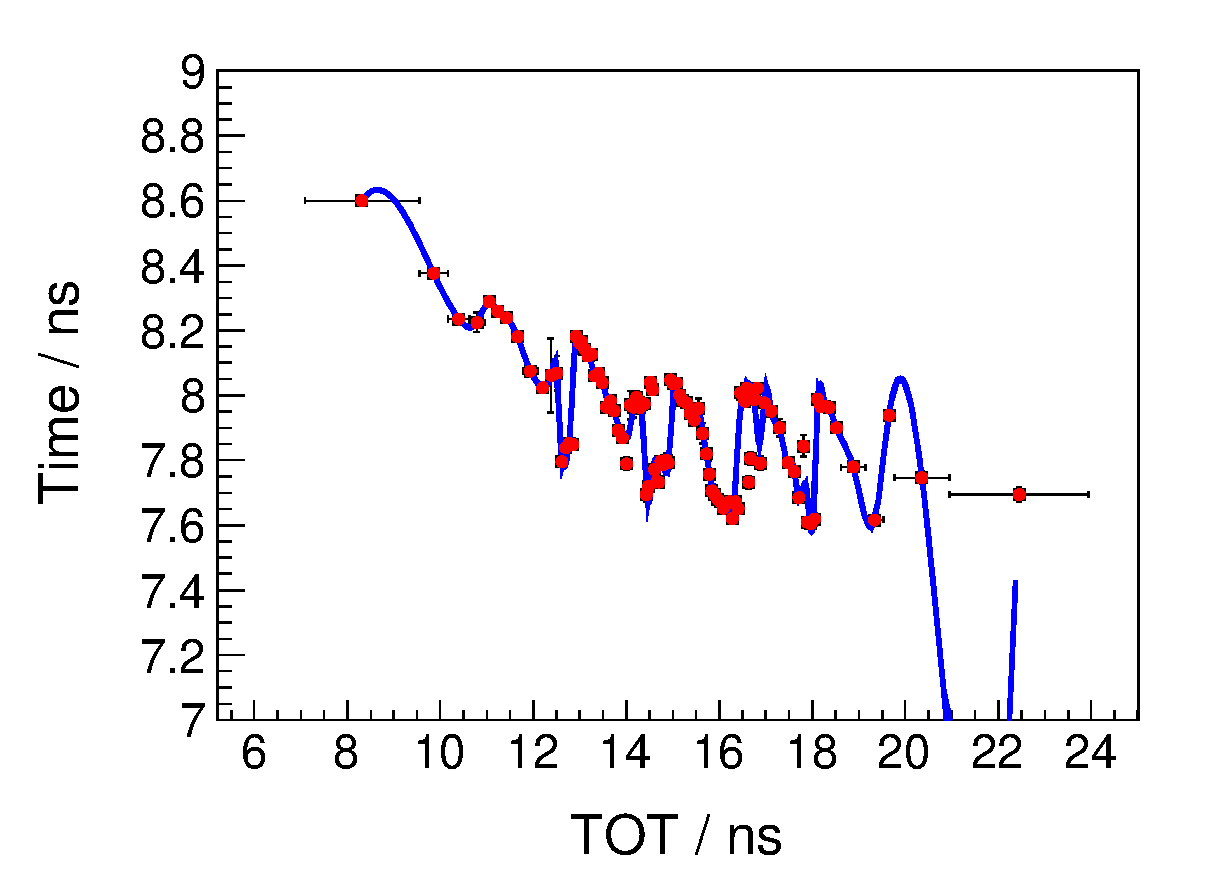
\includegraphics[width=0.95\textwidth]{chap2/double-leftspline.eps}
\subcaption{两个高斯拟合得到的中心值的样条插值}
\label{fig:double-leftspline}
\end{minipage}%
\hfill
\begin{minipage}[!h]{0.5\linewidth}
%\centering
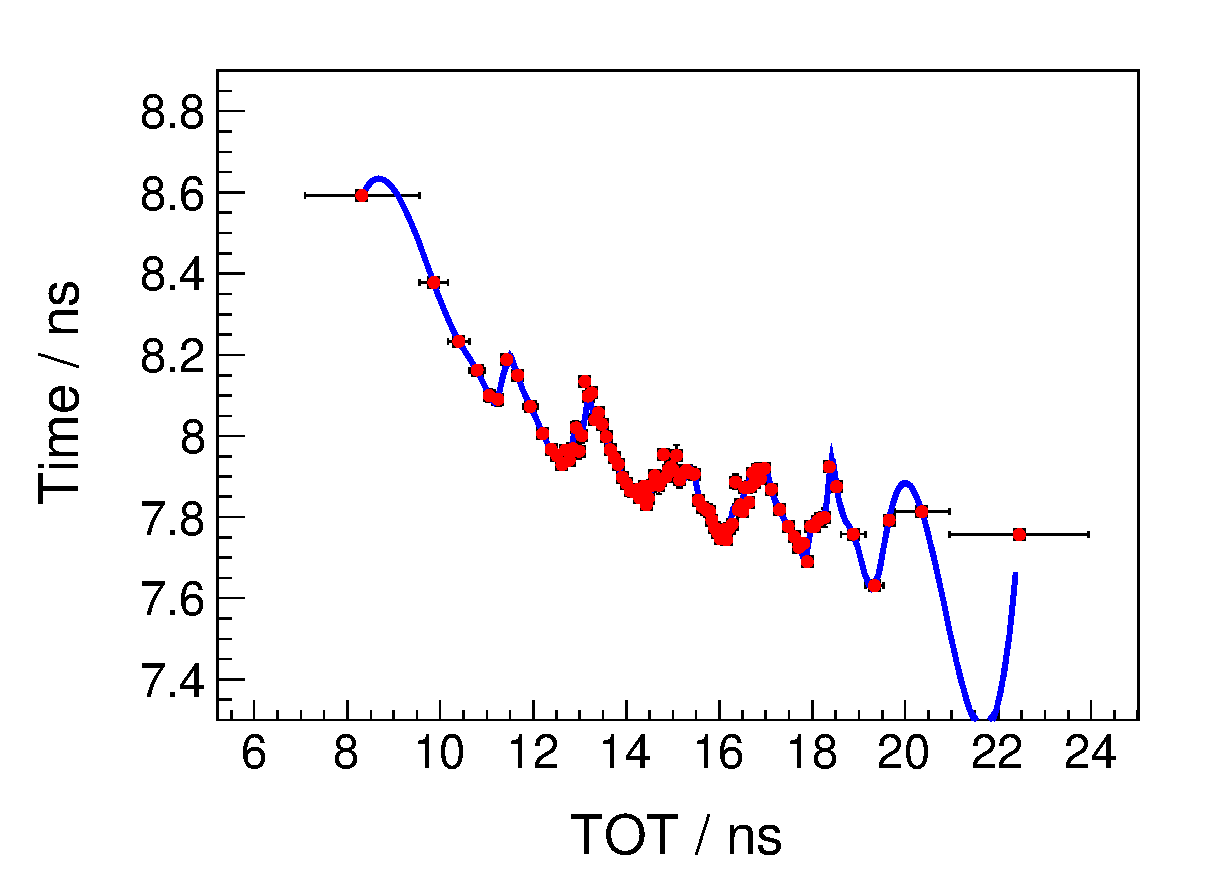
\includegraphics[width=0.95\textwidth]{chap2/single-leftspline.eps}
\subcaption{一个高斯拟合得到的中心值的样条插值}
\label{fig:single-leftspline}
\end{minipage}
\caption{样条插值}
\end{figure}

\subsection{击中位置的修正}
不管上述的哪种方法,插值修正完过阈时间后,时间随击中位置的分布都还有依赖,对此进行一个击中位置的修正,然后得到时间分辨。图~\ref{fig:double-leftspline}~第一种做法得到的时间分辨,为~160ps~;图~\ref{fig:single-leftspline}~第二种做法得到的时间分辨,为~92ps~。这个结果和下一节先修正击中位置,后修正过阈时间的结果相比,差别很大。

分析原因:过阈时间(TOT)的多峰来自反射。一次反射内,时间对过阈时间的依赖近似线性关系,样条插值的光滑性决定不能完全描述这种关系。
\begin{figure}[!h]
\begin{minipage}[!h]{0.5\linewidth}
%\centering
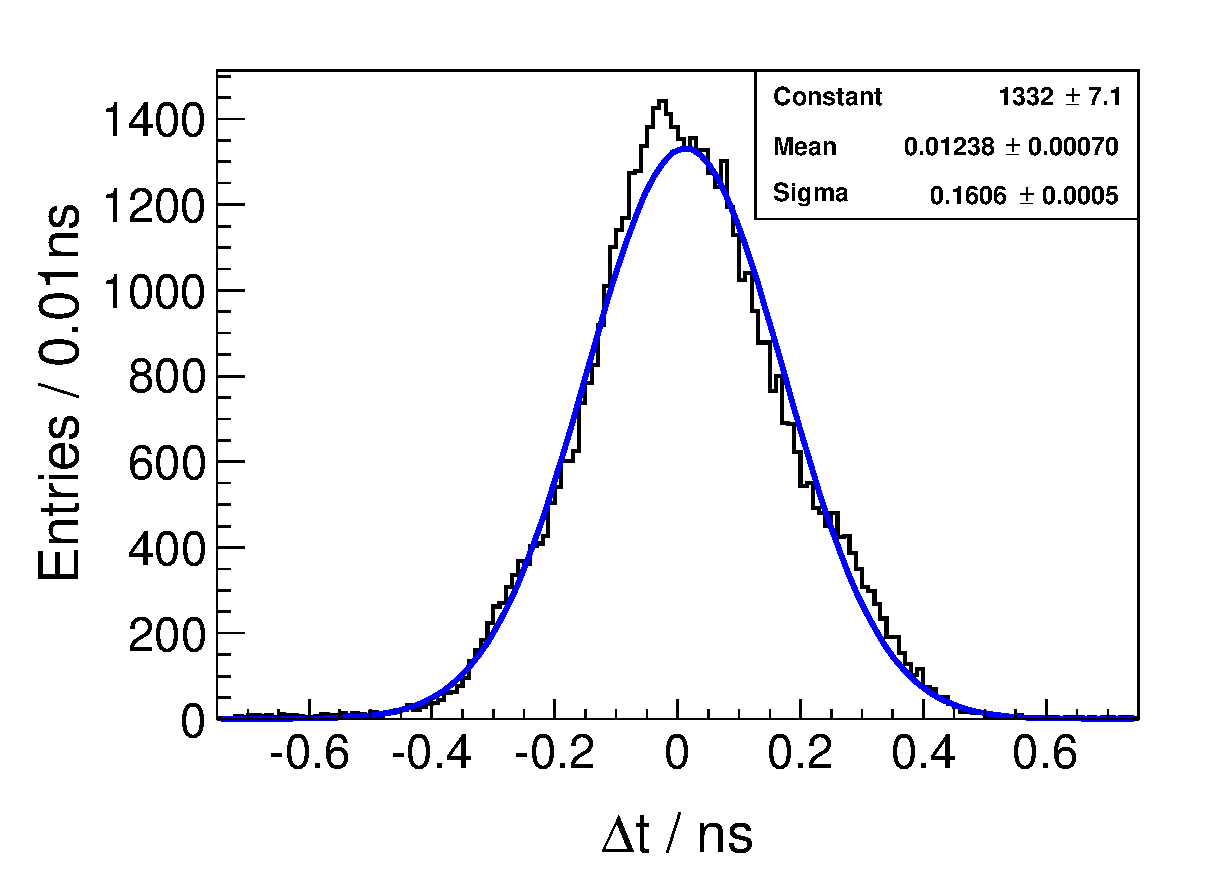
\includegraphics[width=0.8\textwidth]{chap2/double-resolutiongauss.eps}
\subcaption{时间分辨1}
\label{fig:double-resolutiongauss}
\end{minipage}%
\hfill
\begin{minipage}[!h]{0.5\linewidth}
%\centering
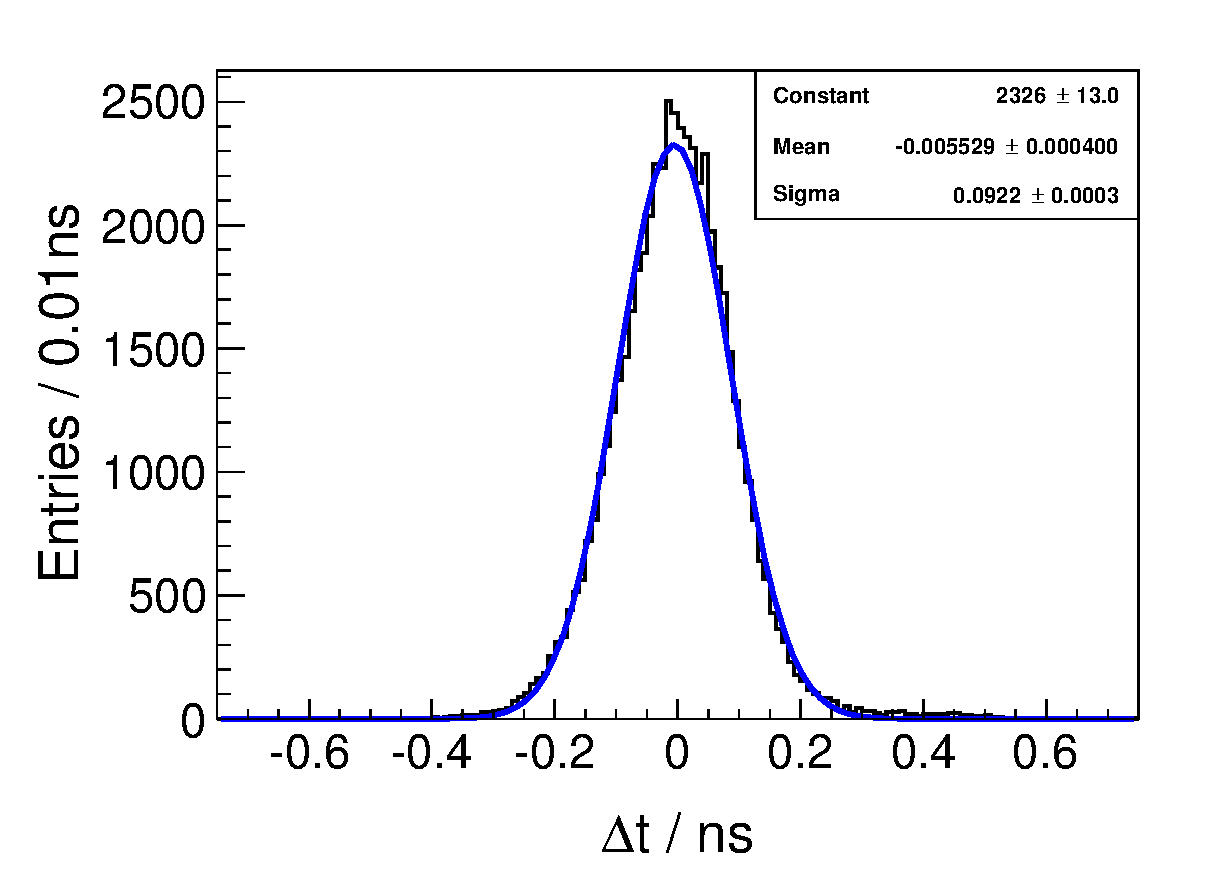
\includegraphics[width=0.8\textwidth]{chap2/single-resolutiongauss.eps}
\subcaption{时间分辨2}
\label{fig:single-resolutiongauss}
\end{minipage}
\caption{时间分辨}
\end{figure}

\subsection{反射问题}


图~\ref{fig:TOT}~是信号的过阈时间。对于一定的阈值,幅度大小不同的信号,对应的过阈时间不同。信号幅度越大,过阈时间也就越大。
图~\ref{fig:reflection}~是~MRPC~读数条的反射问题,分为近端反射和远端反射。由于读数条本身较短,反射信号只是比真实信号时间晚不到1ns,这样导致反射信号和原来的真实信号叠加。测量的过阈时间也就变大了。
正是由于过阈问题和反射问题的存在,导致时间对过阈时间的分布复杂。对时间和过阈时间的关系的研究也刻度研究的重点和难点部分。

\begin{figure}[!h]
\begin{minipage}[!h]{0.5\linewidth}
%\centering
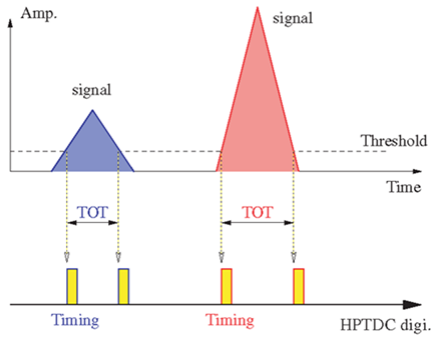
\includegraphics[width=0.8\textwidth]{chap2/TOT.png}
\subcaption{过阈时间~\cite{Shao:2009aa}~}
\label{fig:TOT}
\end{minipage}
\hfill
\begin{minipage}[!h]{0.5\linewidth}
%\centering
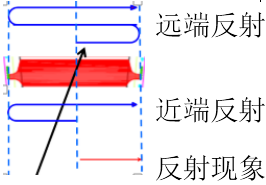
\includegraphics[width=0.9\textwidth]{chap2/reflection.png}
\subcaption{反射问题}
\label{fig:reflection}
\end{minipage}%
\caption{反射问题和过阈时间}
\end{figure}


%%%%%%%%%%%%%%%%%%%%%%%%%%%%%%%%%%%%%%%%%%%%%%%%%%%%%%%%%%%%%%%%%%%%%%%%%%%%%%%
\section{修正击中位置后进行插值}
%%%%%%%%%%%%%%%%%%%%%%%%%%%%%%%%%%%%%%%%%%%%%%%%%%%%%%%%%%%%%%%%%%%%%%%%%%%%%%

\subsection{击中位置的修正后,时间对过阈时间的分布}

图~\ref{fig:q-before}~和图~\ref{fig:q-after}~是击中位置修正前后时间对过阈时间的分布。可以看出,修正完击中位置后时间对过阈时间的折线几乎消失。在此基础上,对过阈时间进行插值拟合。
\begin{figure}[!h]
\begin{minipage}[!h]{0.5\linewidth}
%\centering
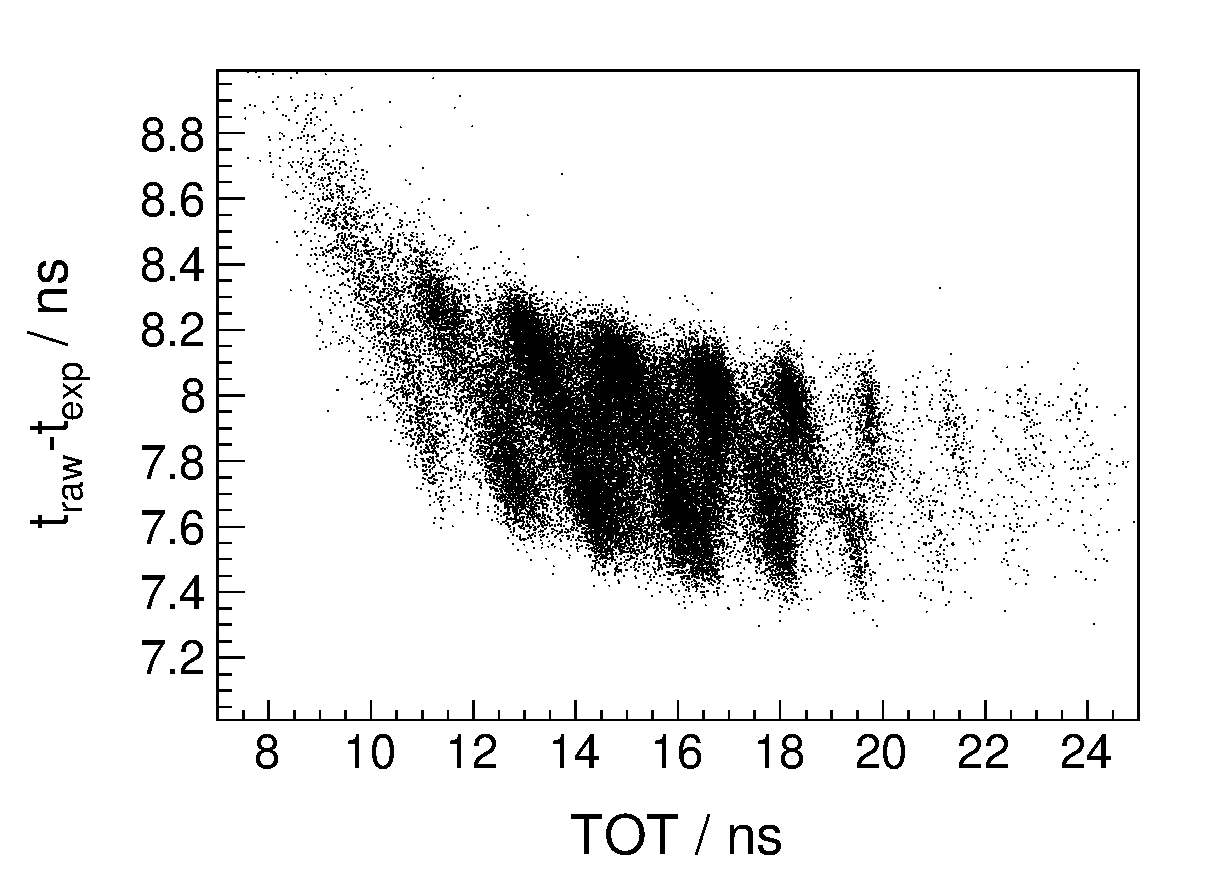
\includegraphics[width=0.9\textwidth]{chap2/q-before.eps}
\subcaption{~Z~修正前}
\label{fig:q-before}
\end{minipage}%
\hfill
\begin{minipage}[!h]{0.5\linewidth}
%\centering
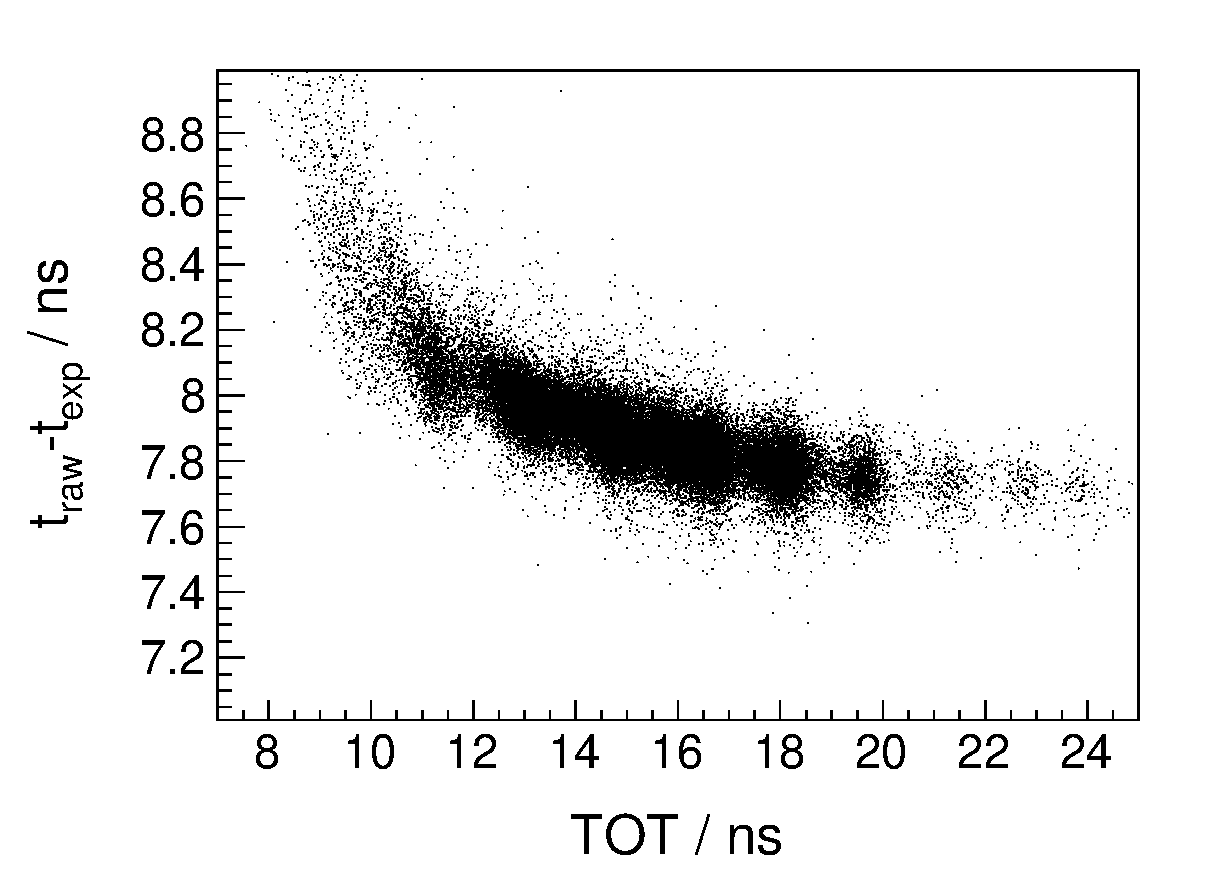
\includegraphics[width=0.9\textwidth]{chap2/q-after.eps}
\subcaption{~Z~修正后}
\label{fig:q-after}
\end{minipage}
\caption{~Z~修正前后时间对~TOT~的分布}
\end{figure}

\subsection{插值}

图~\ref{fig:after-left-spline}~是修正完击中位置后对过阈时间进行样条插值的曲线;图~\ref{fig:resolutiongauss}~是这种方法得到的最终的时间分辨,为~64ps~,比之前先对过阈时间进行插值修正然后对击中位置进行修正得到的时间分辨好。
\begin{figure}[!h]
\begin{minipage}[!h]{0.5\linewidth}
%\centering
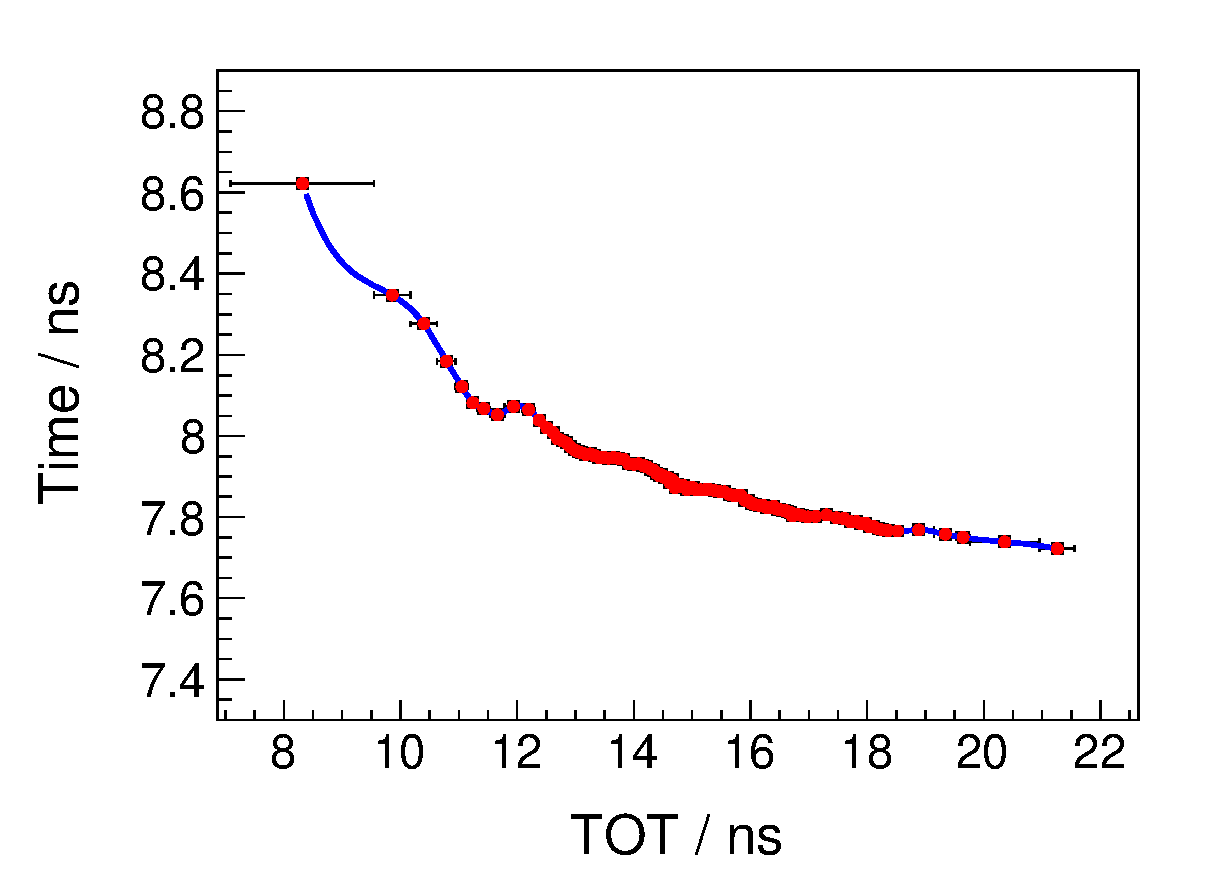
\includegraphics[width=0.9\textwidth]{chap2/after-left-spline.eps}
\subcaption{~Z~修正后对~TOT~进行插值}
\label{fig:after-left-spline}
\end{minipage}%
\hfill
\begin{minipage}[!h]{0.5\linewidth}
%\centering
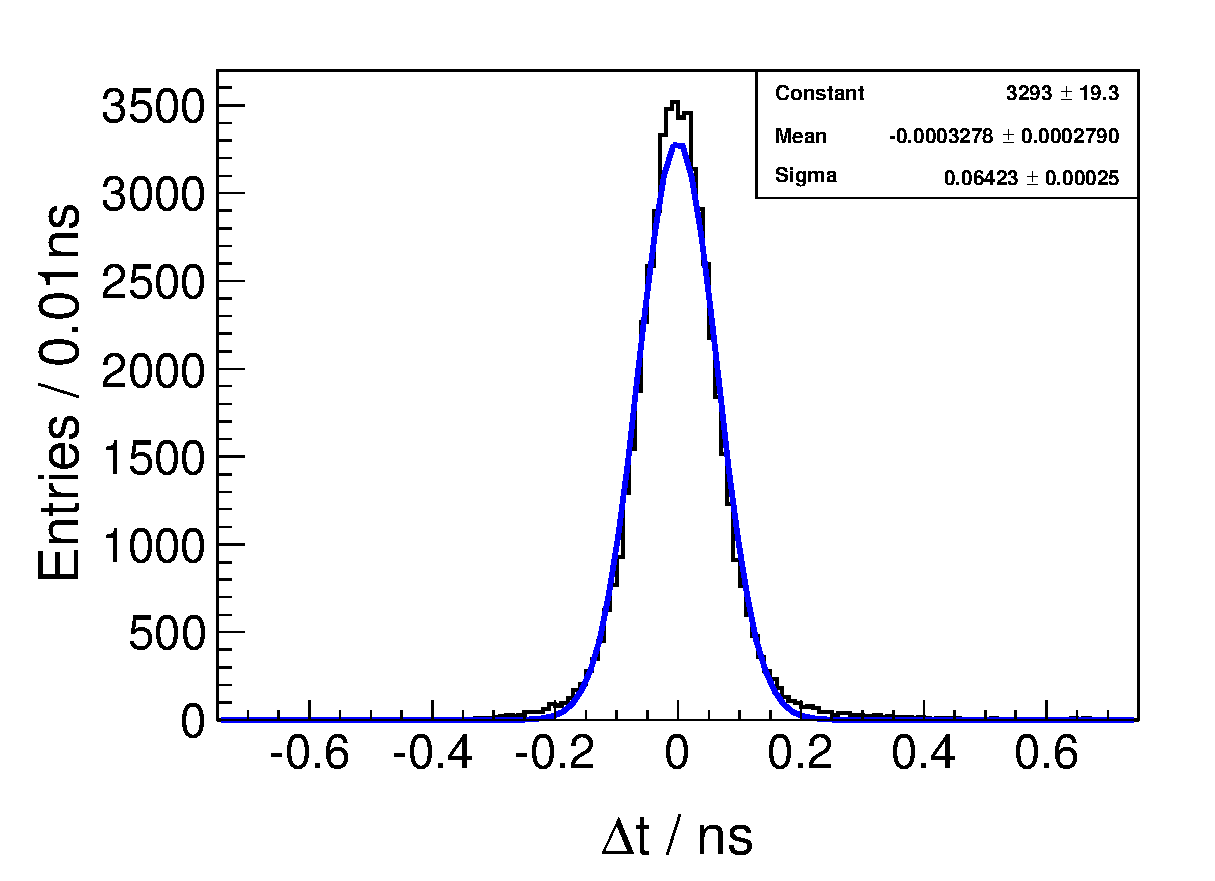
\includegraphics[width=0.9\textwidth]{chap2/resolutiongauss.eps}
\subcaption{时间分辨}
\label{fig:resolutiongauss}
\end{minipage}
\caption{~Z~修正后插值}
\end{figure}

这种对比也说明了先对击中位置进行修正,之后再对过阈时间进行修正是应该采取的修正顺序。

\section{小结}

本章利用样条插值方法,从几个不同的方法对~MRPC~的刻度方法进行了研究和分析。根据不同的方法得到的时间分辨,修正完后时间对击中位置,时间对过阈时间的分布等比较,得出对于~BESIII~实验的~MRPC~刻度应该先对过阈时间进行修正,然后对击中位置进行修正。
插值方法
